\documentclass[conference]{IEEEtran}

\usepackage{float}
\usepackage{graphicx}
\usepackage{xcolor}
\usepackage{flushend}
\usepackage{cite}

\newcommand{\todo}[1]{\textcolor{red}{\textbf{TODO}: {#1}}}

% To make text hidden for review visible: \newcommand{\review}[2]{#1}
\newcommand{\review}[2]{#1}
% add a figure
\usepackage{xcolor,colortbl}
\usepackage{mathpartir}
\usepackage{tikz}
\usepackage{graphicx}
\usepackage{url}
\usepackage{subcaption}   % used for figures in experimental evaluation
\tikzstyle{block} = [rectangle, draw, fill=yellow!30, text width=6em, text centered, rounded corners, minimum height=4em]
\tikzstyle{block2} = [rectangle, draw, fill=green!30, text width=8em, text centered, rounded corners, minimum height=4em]
\tikzstyle{block3} = [rectangle, draw, fill=purple!30, text width=8em, text centered, rounded corners, minimum height=4em]
\tikzstyle{block4} = [rectangle, draw, fill=cyan!30, text width=6em, text centered, rounded corners, minimum height=4em]
\tikzstyle{line} = [draw, -latex']
\usetikzlibrary{arrows,arrows.meta,calc,positioning,backgrounds,fit,shapes,shadows,trees}

\tikzset{%
  thick arrow/.style={
     -{Triangle[angle=120:1pt 1]},
     line width=1.5cm, 
     draw=teal!70
  },
  arrow label/.style={
    text=white,
    font=\sffamily\fontsize{12}{12}\selectfont,
    align=center,
    yshift=-1.25cm
  },
  set mark/.style={
    insert path={
      node [midway, arrow label, node contents=#1]
    }
  }
}

\tikzset{
  basic/.style  = {draw,rectangle,font=\sffamily\fontsize{12}{12}\selectfont}, %text width=2cm, drop shadow},
  root/.style   = {basic, font=\sffamily\fontsize{12}{12}\selectfont, rounded corners=2pt, thin, align=center,
                   fill=orange!30},
  level 0/.style = {basic, font=\sffamily\fontsize{12}{12}\selectfont, thin, align=center, fill=blue!10},
  level 1/.style = {basic, trapezium, trapezium left angle=70, trapezium right angle=110, font=\sffamily\fontsize{12}{12}\selectfont, thin, align=center, fill=green!20},
  level 2/.style = {basic, font=\sffamily\fontsize{12}{12}\selectfont, rounded corners=2pt, thin, align=left,
    fill=yellow!30},
  level 3/.style = {basic, font=\sffamily\fontsize{12}{12}\selectfont, rounded corners=2pt, thin, align=left,
    fill=blue!20, text width=12em},
  level 4/.style = {basic, font=\sffamily\fontsize{12}{12}\selectfont, thin, align=center, 
    fill=green!30},
  level 5/.style = {basic, font=\sffamily\fontsize{12}{12}\selectfont, thin, align=center, 
    fill=orange!30},
  level 6/.style = {basic, rectangle, font=\sffamily\fontsize{12}{12}\selectfont, thin, align=center, 
    fill=cyan!20},
   boxaround/.style={draw=violet, font=\sffamily\fontsize{12}{12}\selectfont, thick, dashdotted,
     inner sep=0.8em},
 >=latex
}

\usepackage{paralist}
\usepackage{boxedminipage} %proof rules
\usepackage{booktabs} %proof rules
\usepackage{chngcntr}
\counterwithout{figure}{section}

\begin{document}


\title{Towards Explainable Compositional Reasoning}

\author{\IEEEauthorblockN{
		Isaac Amundson, Amer Tahat, David Hardin, and Darren Cofer}
	\IEEEauthorblockA{Applied Research and Technology, Collins Aerospace, USA\\
		{\{first.last\}@collins.com}}
	}



\maketitle

\begin{abstract}

Formal verification tools such as model checkers have been around for decades.  Unfortunately, despite their ability to prove that mission-critical properties are satisfied in both design and implementation, the aerospace and defense industry is still not seeing widespread adoption of these powerful technologies. 
%
Among the various reasons for slow uptake, difficulty in understanding analysis results (i.e., counterexamples) tops the list of multiple surveys.
%
In previous work, our team developed AGREE, an assume-guarantee compositional reasoning tool for architecture models.  Like many other model checkers, AGREE generates potentially large counterexamples in a tabular format containing variable values at each time step of program execution up to the property violation, which can be difficult to interpret, especially for novice formal methods users.
In this paper, we present our approach for achieving \textit{explainable} compositional reasoning using AGREE in combination with generative AI.  Our preliminary feasibility results indicate this technique works surprisingly well, and have encouraged us to expand this approach to other areas in explainable proof engineering.  
	

\end{abstract}

\vspace{12pt}
DISTRIBUTION STATEMENT A. Approved for public release: distribution unlimited.

\section{Introduction}
\label{sec:introduction}
PROVERS

INSPECTA


\section{Explainable AGREE}
\label{sec:agree}
\subsection{Overview}

% Overview

AGREE provides a formal contract language for specifying \textit{assumptions} (i.e., expectations on a component's input and the environment) and \textit{guarantees} (i.e., bounds on a component's behavior). AGREE uses a k-induction model checker to prove properties about one layer of an architecture using properties allocated to subcomponents. 



%AGREE Spec language?

AGREE Counterexamples





Component interfaces– The output guarantees of each component must be strong enough to satisfy the input assumptions of downstream components. 

Correctness of implementations– The input assumptions of a system along with the output guarantees of its sub-components must be strong enough to satisfy its output guarantees.



\subsection{Making Counterexamples Actionable} 
In the following sections, we introduce AGREE-Dog, an interactive conversational copilot powered by GPT-4o (omni) multi-modal generative AI, specifically developed to assist AGREE users in identifying the root causes of counter-examples generated by AGREE and to support the subsequent model repair process. It is designed to be user-friendly and integrated with the OSATE IDE (see Figure \ref{fig:AGREEDOG}). \footnote{In the figure Figure \ref{fig:AGREEDOG} AGREE-Dog is a specific instance of the INSPECTA-Dog toolset, where users can select the copilot's identity. This paper focuses on the AGREE-Dog instance, while other instances of INSPECTA-Dog are beyond the scope of this discussion.}

\begin{figure*}[htbp]  
    \centering
    \includegraphics[width=\textwidth]{AGREE-Dog.png}  % Use \textwidth for full two-column width
    \caption{AGREE-Dog, acting as a copilot to OSATE, provides explanations for the counter-example generated by the AGREE tool for the AADL model \texttt{Car.aadl}.}
    \label{fig:AGREEDOG}
\end{figure*}


 We detail our methodologies for addressing the primary challenges we have encountered, present our key findings, and discuss the current limitations and directions for future work. To elucidate these challenges, we use the \texttt{Toy\_Integers.aadl} and \texttt{car.aadl} models as two running examples throughout the paper.

\subsection{Contextual Prompt Constraints Problem}

The GPT-4o generative multi-modal model exhibits significant power in translating human instructions into code and vice versa, particularly when the language in question has been part of its pre-training data and there exists a substantial open-source code base, such as C or Python. However, this capability comes with the drawback of potential hallucinations. Since AGREE is not as widely adopted as languages like C or Python, this problem is exacerbated. Consequently, one of the primary challenges we encountered involved the explainability of counter-examples due to the absence of relevant context.
\subsubsection{Dog Retrieval-Augmented Generation (RAG) System}

 To mitigate this problem we designed AGREE-Dog RAG system we implemented the system to be dynamic, allowing it to adjust its context based on user inquiries. 
%In particular, it reads the content of the current working \texttt{AADL} file enclosd between two terminators, analyzes the import chain, and practicaly retrieves the necessary context from these files (see Figure \ref{car}). %This approach is particularly effective in extracting relevant information from potentially large repositories.

Despite GPT-4o's 128k token capacity, which we estimate can accommodate several thousand lines of \texttt{AADL} code in a single prompt, uploading an entire repository's contents can be prohibitively expensive and may well exceed the the prompt token limitations. Therefore, we implemented a practical two-step optimization technique that meets our current needs.

First, AGREE-Dog RAG system reads the current working file, then it parses the file's import chain, extracting only the files on this chain. This step significantly reduces the initial prompt size, see Figure \ref{fig:AGREEDOG}.  
%
The second optimization addresses another practical requirement: handling parts of the repository that may have been included in the model's pre-training data, such as core libraries. To manage this, AGREE-Dog's RAG system applies a filtering technique to the file names, guiding the system to ignore certain files, such as standard libraries, and retain user-defined files. This approach further reduces the initial prompt size to include only files that the model has not previously encountered. Finally, the user inputs are automatically incorporated into the extracted context from the current file and its import chain, allowing for more accurate responses to user inquiries.

This approach significantly mitigates contextual constraint-based hallucinations that can arise from the absence of AADL model specifications. However, it does not address the absence of the counter-example itself or the lack of guidance on the critical system requirements that should be preserved during the model repair process.
 

\subsection{Model Repair Problem}

Given that counter-examples are generated interactively and may not be included in the initial context, we dynamically extend the AGREE-Dog RAG system. This allows users to upload an AADL model file along with the counter-example in a CSV or Excel file %(Figure \ref{fig:AGREEDOG2}).
Upon submission, the copilot provides a detailed, step-by-step explanation of the counter-example, identifies its root cause(s), and suggests potential solutions, (Figure \ref{fig:AGREEDOG}). 


However, a significant challenge encountered was that these explanations and suggested alternatives could include two types of hallucinations, both syntactic and semantic. The former are typically minor and can be detected and resolved using a multi-shot approach. The latter are more problematic, as the AGREE-Dog system might suggest altering a guarantee requirement, which could successfully remove the counter-example but risk violating core system requirements that should remain unchanged, we refer to this problem by \textit{Model Repair Problem}. 


\subsubsection{Requirements for Counterexample Explanations}

To mitigate the Model Repair Problem, we configured AGREE-Dog to generate solutions that conform to a predefined set of system requirements written in natural language, which are uploaded via an Excel sheet or CSV file or directly included in the context. 

\begin{figure}[t]  
    \centering
    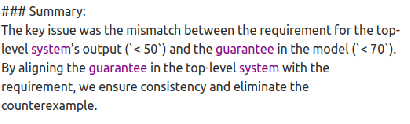
\includegraphics[width=0.95\columnwidth]{REQ-AWARE-REF.png}  % Use \columnwidth for single column width
    \caption{AGREE-Dog Refined Explanations Using a Requirements File. \texttt{Toy\_Integer.aadl}.}
    \label{fig:REQ-AWARE-EXPL}
\end{figure}


As a result, AGREE-Dog was able to more accurately identify the root cause and suggest appropriate solutions as demonstrated in Figure \ref{fig:REQ-AWARE-EXPL}.

%For instance, in the \texttt{Toy\_Integer} model, a basic requirement like \texttt{guarantee\_3} (\texttt{certain\_variable < 50}) might suggest adding to component C. While this could eliminate the counter-example, it may not align with the intentions of the system engineers and domain experts, leading to what we consider a candidate for requirement absence hallucinations.

This refinement significantly enhanced the accuracy of AGREE-Dog’s recommendations.


\subsection{Preliminary Results and Conversational Quality Assessment Problem}
 
Our initial evaluations were conducted manually, focusing on AGREE-Dog's ability to accurately identify the cause of counter-examples, repair the model, and ensure compliance with the uploaded requirements. The system was evaluated on two case studies. The first case study involved a toy model, \texttt{Integer\_Toy.aadl}, while the second dealt with a larger model that imports several files, totaling 7 files and approximately \texttt{xx} lines of code. AGREE-Dog successfully identified the root cause of all counter-examples for the specified guarantees (13 out of 13) on the first attempt, demonstrating a high degree of accuracy.

However, these manual evaluations, highlighted the need for greater automation. Consequently, we are developing a more automated evaluation system to enable testing on more realistic and complex use cases, that autoamte the evaluation workfollow as shown in Figure ~\ref{fig:CQAS}.
 

\begin{figure}[htbp]
\centering % Still centering the figure
\hspace*{-1cm} % Shift the entire figure to the left by 1 cm
\resizebox{0.95\columnwidth}{!}{ % Keep the size slightly below the full column width for better fit
\tikzstyle{root} = [rectangle, fill=white!3, text width=4.5em, text centered, minimum height=2em, node distance=.10cm]
\tikzstyle{block} = [rectangle, draw, fill=blue!3, text width=5.3em, text centered, minimum height=2em, node distance=.40cm]
\tikzstyle{block1} = [rectangle, draw, fill=red!3, text width=7em, text centered, minimum height=2em, node distance=.5cm]
\tikzstyle{block2} = [rectangle, draw, fill=gray!3, text width=6em, text centered, minimum height=2em, node distance=.5cm]
\tikzstyle{block3} = [rectangle, draw, fill=green!10, text width=8em, text centered, minimum height=2em, node distance=.55cm]
\tikzstyle{line} = [draw, -latex']

\begin{tikzpicture}[auto, node distance=2cm,>=latex']
    % Place nodes
    \node [root] (root1) {};
    \node [block1, right=of root1] (interactions) {\texttt{\textbf{AGREE-Dog}} User-System Interactions};
    \node [block2, below=of interactions] (history) {Conversation History Management};
    \node [block2, right=of history] (lemma) {Model-Repair Multi-Shots Dictionaries};
    \node [block2, right=of lemma] (quality) {Collecting Quality Metrics Automatically};
    \node [block3, above=of quality] (stat) {\textcolor{blue}{Statistical Analysis and Visualization}};

    % Draw edges
    \path [line] (root1)  (interactions);
    \path [line] (interactions) -- (history);
    \path [line] (history) -- (lemma);
    \path [line] (lemma) -- (quality);
    \path [line] (quality) -- (stat);
\end{tikzpicture}
} % End of resizebox
\caption{AGREE-Dog Conversation Quality Assessment System (CQAS) workflow.}
\label{fig:CQAS}
\end{figure}

We are in the process of selecting a golden set of examples from a formally verified library we developed previously, and constructing a testing set by introducing deliberate violations. These examples are uploaded to the AGREE-Dog system to evaluate its ability to correctly identify the root causes. While AGREE-Dog has demonstrated initial success in this area, model repair evaluation remains a more complex challenge. This is because repairing models can result in multiple solutions, particularly for more intricate use cases. One of the key limitations is the system's ability to consistently remove counter-examples while ensuring compliance with the specified requirements. To address these issues, we are developing a toolset aimed at measuring the system’s convergence towards the correct semantics of the golden examples, within a few-shot learning context. This remains an ongoing challenge that we are working to address in our future work. %extend our prior research from the \cite{coqDog} paper to improve AGREE-Dog's performance in these areas


%\subsection{Preliminary Results}




%\section{Related Work}
%\label{sec:related-work}
%\input{relatedwork}

\section{Conclusion}
\label{sec:conclusion}
Summary

Future Work:

Use AgreeDog to generate AGREE spec statements?

AgreeDog integration with OSATE

Assurance Dashboard

Metrics capture

%\section{Acknowledgment}
%This work was funded by DARPA contract XXXXXXXXX. The views, opinions and/or findings expressed are those of the authors and should not be interpreted as representing the official views or policies of the Department of Defense or the U.S. Government.

\bibliographystyle{IEEEtran}
\bibliography{biblio}

\end{document}
